%\usepackage{natbib}

\chapter{Introduction}

%\paragraph*{Why was this topic important to investigate?}
\paragraph{}
Deep next generation sequencing, producing millions of short RNA reads per sample,
has become a great asset for tasks such as transcriptome abundance estimation, and
assembly as well as providing a rich database of information over hundreds of thousands of individuals
with associated meta-data and extensive variation. The low-cost and simple protocol for
producing short reads has provided the community with massive collections of raw sequence samples.
In addition to the large collections of raw sequence samples,
there exist large databases of assembled genomes and transcriptomes
due to computational advancements in sequence assembly
using RNA reads specifically in the domain of metagenomics.
There has been a lot of effort and research in organizing and indexing these databases
and extracting information from them efficiently~\cite{paten2017genome}.
Such indices have been used in various computational
and biological applications such as alignment and mapping,
genome and transcriptome abundance estimation and differential expression,
and genome and transcriptome assembly and variation/isoform detection.
In addition to all these applications, these databases themselves are a great resource
of information to find out sequence-based novelties, differences, disparities and abnormalities
across different species, individuals, tissues, or even single cells.
To extract and analyze this information, the role of a dynamic and efficient search index
over such big databases of (short raw and long assembled) sequences
with the ability of quick queries is essential.
The amount of research done in the past decade on building indices over
the genomic and transcriptomic sequences and the tremendous use of those tools by biologists
in their analyses adds to the importance of this matter and its usefulness.

%\paragraph*{What did we know about this topic before I did this study?}
\paragraph*{}
While there have been a wide variety of tools developed
for indexing and querying large collections of sequences in the past
~\citep{li2008mapping,langmead2009ultrafast,li2009fast,hach2010mrsfast,langmead2012fast,li2013aligning,liao2013subread,dobin2013star,kim2015hisat},
we can divide them into two main categories of linear- and graph-based indices.
In the linear-based approaches, the series of sequences are put together and treated as one large text
and then indexed based on well-known data structures for indexing large-text sequences
such as FM-index or suffix arrays
~\citep{langmead2009ultrafast,li2009fast,langmead2012fast,li2013aligning,dobin2013star,kim2015hisat}.
These indices (also called full-text indices) are usually very small, compared to the size of the
raw data they index but can be slow to query.
On the other hand, the graph-based indices make use of factoring out the repeats in the sequences
to reduce the size of the index and provide faster queries.
In these approaches, a sequence is
splitted into sub-sequences of size k (called a \kmer) where each \kmer is presented only once
in the whole index.
Yet, although much faster than the full-text approaches, they are often orders of magnitude larger.
Therefore, having an index with a balance between the memory and query time
is still a continuing challenge that requires solving computational problems by applying
existing algorithms in other areas of computer science or developing new ones.

One of the mostly used types of graph in graph-based indexing is the \dbg
and its variants, the \longcdbg (cdbg), the \compdbg, and the compacted \longcdbg.
I’ve worked on two particular problems. The first is succinct representation of membership information
in a \longcdbg, and the second is efficient indexing for \kmers
in a compacted \longcdbg.
Below I provide a brief overview of previous works on graph-based representation,
along with common use cases of the various algorithms and methods developed.

\section{De Bruijn Graph}
\label{subsec:dbg}
A \dbg (dbg) is a directed graph representing a set of sequences.
This type of graph has two variants, node-centric and edge-centric.
In the edge-centric \dbg, each directed edge is a unique substring of length $k$ in the sequence set,
which we call a \kmer. Each edge has a prefix overlap of $k-1$ bases with the source node
and a suffix overlap of length $k-1$ with the destination node~\cite{paten2017genome}.
Figure~\ref{fig:dbg-a} shows a simple \dbg for a sample with one string.
This type of graph is designed so that by having a walk through edges and
putting all edges next to each other with overlaps of $k-1$,
we are able to build the reference sequence, such as a gene or transcript,
as shown in~\ref{fig:dbg-b}. Ofcourse it is worth noting that such ``perfect assembly''
is not always possible due to sequencing errors, repeats, and other complexities that come in the way.
In the node-centric variant of a \dbg, each node represents a \kmer,
connected by overlapping strings in the same way.

\begin{figure}
    \centering
    \begin{subfigure}{.5\textwidth}
        \centering
        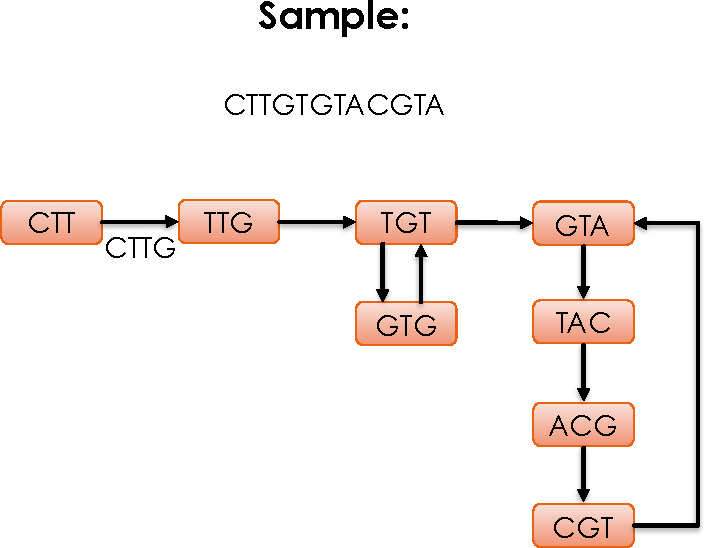
\includegraphics[width=\linewidth]{figs/dbg1-cropped.pdf}
        \caption{de Bruijn graph for a sample with one sequence.}
        \label{fig:dbg-a}
    \end{subfigure}%
    \begin{subfigure}{.5\textwidth}
        \centering
        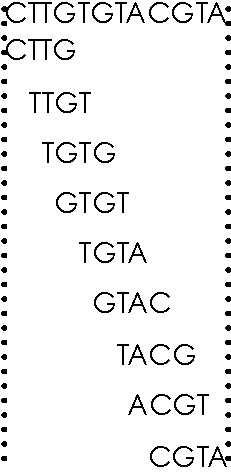
\includegraphics[width=.4\linewidth]{figs/dbg2-cropped.pdf}
        \caption{This example shows how one can reconstruct the reference sequence
        having a walk through nodes and edges in a de Bruijn graph and taking care of overlaps.}
        \label{fig:dbg-b}
    \end{subfigure}
    \caption{Building a de Bruijn graph and reconstructing the reference sequence from it}
    \label{fig:dbg}
\end{figure}

The \dbg is a useful structure for indexing a reference or set of sequencing reads
because it enables fast querys.
One drawback is that for the $k-1$ overlaps between consequent edges,
the original data structure is very space-inefficient. For example,
ABYSS~\cite{simpson2009abyss} represents the \dbg as a hash table with each \kmer
as the key and a byte keeping all the connections to other nodes as its value.
It needs $1$ bit to show the existence of each of the edges in forward or reverse-complement case
(as we have four characters in our alphabet, we can expand the current node
to reach to the next one in at most four different ways in forward direction).
The space such a data structure takes is $\abs{E_s}(\frac{k}{4}+1)\frac{1}{\gamma}$ bits
where $\gamma \leq 1$, is the hash table loading factor.
This storage is considerably large for even one genome data set,
such as the human genome (starting from 40GB while depending on the loading factor can grow to 100GB or more).
Yet, a few different data structures and algorithms have been proposed to reduce the size of a \dbg
and represent it efficiently. One category of these data structures use the Bloom Filter~\cite{}
to represent a \dbg~\cite{pell2012scaling,salikhov2013using,chikhi2012space,chikhi2013space,holley2016bloom}.
Other than these, there are a few proposed representations
that rely on succinct data structures~\cite{gbmp2014sea}
and rank and select operations including the original work by Conway and Bromage~\cite{conway2011succinct}
and later the work in~\cite{BoweOn12} that is called the BOSS representation of \dbg from the authors’ initials.
BOSS is an efficient, edge-centric representation of \dbg that takes around 3 bits per \kmer,
which is considerably smaller than the hash table representation.
This representation provides a mechanism for navigation through the \dbg
and also an interface to interact and get access to the ID of each \kmer.
In section~\ref{chap:rainbowfish}, I explain in more detail, our work on the color representation
for a \dbg built on top of the BOSS structure, using the interface it provides.


\subsection{Compacted \dbg}
\label{subsubsec:cdbg}
The main advantage of a \ccdbg is being more space-efficient compared to the
classic representation of the \dbg due to the nodes representing
paths with no branches rather than \kmers.
The process of compacting the \dbg is meant to merge all \kmers in a non-branching path
in the \dbg with outgoing and incoming degrees of
one into a single node which is called a \emph{unitig}.
The output of this step is called a \compdbg,
that connects these unitigs and is a variant of the original \dbg
with unitigs as nodes rather than the \kmers.
This can be used in the same way as a \dbg for different downstream applications,
such as mapping, alignment, variant detection, etc.
This method reduces memory by eliminating the great amount of overlaps of $k-1$ bases
repeated in consequent \kmers.
For instance, the output node after merging two consequent nodes in a node-centric \dbg
with overlap of $k-1$ would be a unitig of length $k+1$ where the node starts with the first base in the source node,
continues with the $k-1$ overlapping bases and ends in
the last base of the destination.
This compaction step can have a great impact on reducing the memory
and is very useful in cases that we are dealing with repeat-heavy sequences~\cite{liu2016debga}.
Recently, researchers have designed and implemented algorithms for building
a \ccdbg directly from raw data instead of building the memory-inefficient \dbg first
and then compacting it~\cite{minkin2016twopaco,chikhi2016compacting}.
However, indexing a \ccdbg is still a challenge that needs further investigation.

%\paragraph*{How will this study advance new knowledge or new ways of understanding?}
\paragraph*{}
%\fatemeh{Is this still true?}
So far, we know of two other tools, kallisto~\cite{Bray2016Kallisto}
, deBGA~\cite{liu2016debga} and deSALT~\cite{} that are used for indexing \ccdbgs.
Although these tools are very efficient in searching for a \kmer, the memory they need is large,
so that in the case of very large datasets their memory exceeds the limits of a moderate server.
In section~\ref{chap:pufferfish}, we propose a memory-efficient indexing data structure
for a \ccdbg that has an asymptotically constant \kmer lookup time.
We first use one of the existing tools that we discussed earlier to build the \ccdbg~\cite{minkin2016twopaco}.
Later in the same section, we explain our novel data structure to index such \ccdbgs
while keeping a balance between space and query time.
One great advantage of a specific variant of our indexing structure (sparse indexing)
is the flexibility that it provides by giving the option of trading time for space
by means of a tunable parameter.

\subsection{Colored \dbg}
A \cdbg is a generalized form of a \dbg that allows representing multiple samples
in one unified graph while keeping the identity of (and information specific to) each sample~\cite{Iqbal2012Novo}.
The samples may be the result of different experiments for the same species, known variants of the same sequence,
or different sequencing samples. By counting all of the samples together as one
and building a \dbg from them we will lose the variations happening across samples.
Colored de Bruijn graphs were originally proposed by Iqbal et. al~\cite{Iqbal2012Novo}
in a tool named \emph{cortex}, useful for variant discovery and genotyping.
Each sample is represented with a unique color in a \cdbg and
hence all the \kmers coming from that sample will carry that color with them.
To be exact, each \kmer or edge in a \cdbg has a color set showing all the samples
that this \kmer has appeared in.
Maintaining each color separately, we can differentiate between bubbles that are induced by \emph{repeats}
when we see the coverage evenly distributed along different paths from \emph{errors}
where one side of the branch has a low coverage~\cite{Iqbal2012Novo}.
There are other data structures implemented in tools such as BFT~\cite{holley2016bloom}
and VARI~\cite{MuggliBoNo17} for representing and processing \cdbgs.
However, in most of the cases the color representation is the dominant part in the total space
the \cdbg takes compared to the small portion that is taken by the \dbg representation itself.

%\paragraph*{How will this study advance new knowledge or new ways of understanding?}
\paragraph*{}
In chapter~\ref{chap:rainbowfish} we propose a succinct data structure to represent colors in a \cdbg
paired with any \dbg representation that provides a unique index for each \kmer.
We theoretically prove the succinctness of our data structure and compare our space and query time results
with VARI which uses a similar API to construct the index and find bubbles in the \cdbg.

\section{Sequence Search}
\label{subsec:seqsearch}
The ability to issue sequence-level searches over publicly available databases
of assembled genomes and known proteins has played an instrumental role in many
studies in the field of genomics, and has made BLAST~\citep{Altschul1990BLAST}
and its variants some of the most widely-used tools in all of science.
However, these indices are defined over a database of reference sequences.
Yet, the vast majority of
publicly-available sequencing data (e.g., the data deposited in the
SRA~\citep{Kodama2011sequence}) exists in the form of raw, unassembled
sequencing reads for which the reference-based indices are not
a suitable choice. First, because they do not
scale well as the amount of data grows to the size of the  SRA (which today is
$\approx 4$ petabases of sequence information) and second, because relatively long queries (e.g.,
genes) are unlikely to be present in their entirety as an approximate substring
of the input in the raw sequence reads (which are usually less than 200 bases long).

This problem was first introduced and tackled by~\citet{Solomon2016Fast}.
They introduced an algorithm that enables an
efficient type of search over thousands of sequencing experiments.
Specifically, they re-phrase the query and each separate experiment of reads
in terms of \kmer set membership in a way
that is robust to the fact that the target sequences have not been assembled.
The resulting problem is coined as the \emph{experiment discovery} problem,
where the goal is to return all experiments that contain at least some
user-defined fraction $\theta$ of the \kmers present in the query string.
The space and query time of the SBT structure has been further improved
by~\cite{Solomon2017Improved} and~\cite{Sun2017Allsome}.
However, scaling this representation is still an issue
which leads us to the next tool that we've worked on called \mantis.

%\paragraph*{How will this study advance new knowledge or new ways of understanding?}
\paragraph*{}
In chapter~\ref{chap:mantis}, we introduce \mantis,
a space- and time-efficient index for searching sequences in large
collections of experiments which is based on \cdbgs.
The ``color'' associated with each \kmer
in a \cdbg is the set of experiments in which that \kmer occurs. We
use an exact \cqf~\cite{PandeyBeJo17a}, an AMQ structure~\cite{}
to store a table mapping each \kmer to a color ID,
and another table mapping color IDs to the actual set of experiments
containing that \kmer and achieve 20$\%$ times smaller memory,
and up to $108X$ improvement in query time compared to the previous representations.

\section{Reference-based and Reference-free Indexing}
\label{subsec:indexing}
Aligning and mapping sequence reads to a reference genome or transcriptome
is an important and unavoidable step
of many pipelines in genome and transcriptome analysis.
For almost all types of quantification and gene and RNA sequence expression analyses,
we first need to align short reads to the reference gene and transcript. However,
in most of the analyses, this step is the time-consuming bottleneck.
To speed up the alignment process, researchers have developed a seed-and-extend methodology
to first find an exact match to a seed from read and continue aligning from that point.
Most of the popular indices are to be used for the seed-and-extend approach including both
\kmer-based indices such as~\cite{liao2013subread}
%\fatemeh{change this to two other kmerbased ones}
and linear self indexing ones such as Bowtie2~\cite{langmead2012fast}
and BWA-MEM~\cite{li2013aligning} that make use of Borrows Wheelers Transform,
or suffix array based indices such as STAR~\cite{dobin2013star}.
As mentioned earlier, there have been recent efforts to extend both approaches to the context
of indexing different types of sequence graphs~\cite{paten2017genome},
with tradeoffs between space and time efficiency.
On the succinct self-index side, one notable example is gramtools, the tool in which the graph itself
is represented as a modified BWT~\cite{maciuca2016natural}.
For the recently developed \kmer lookup based approaches, however,
it is more prevalent to use graphs as the underlying data structure.
The examples are tools like deBGA~\cite{liu2016debga},
genomeMapper~\cite{schneeberger2009simultaneous}, and BGREAT~\cite{limasset2016read}.

%\paragraph*{How will this study advance new knowledge or new ways of understanding?}
%These efforts are interesting, in part, for the specific representation of \emph{unitigs}
%in \ccdbgs explained in section~\ref{subsubsec:cdbg}.
%The absence of duplicate \kmers in the unitig set allows efficient indexing of these \kmers
%with a minimum perfect hash function (MPHF)~\cite{limasset2017fast}.
%In chapter~\ref{chap:pufferfish}, we present pufferfish, an efficient indexing representation of the \ccdbg
%annotated with information like color, position, orientation, and frequency of each \emph{unitig}.
%We present two variants of the pufferfish data structure, dense and sparse.
%The first is optimized for fast queries
%and the second provides the user with the ability to trade off space for speed in a fine-grained manner.

\section{Ongoing and Proposed Work}
My future thesis plan lies in two different but related directions
as the continuation of my previous projects that I will work on in parallel.
One of the main usecases of Pufferfish as an index with moderate memory
and efficient factorization of repeats of sequences is in indexing thousands of genomes
in the metagenomic analyses. In chapter~\ref{chap:pufferfish}, we even investigate
the idea by building an index over thousands of E. coli genomes.
One can now use it for metagenomic abundance estimation which is one of the projects
I propose to work on as a showcase for Pufferfish and its usefulness.
One of the main challenges in metagenomic abundance estimation is the large number of false positives
in reporting the abundance for species because of the high similarity of sequences
and absence of references from the database.
I propose Cedar, a metagenomic abundance estimation tool on top of the Pufferfish index.
Having worked with different types of sequences in the past four years,
I have a good perspective about different types of gene and transcript sequences.
Therefore, I intend to use algorithms and methodological approaches successful there to
improve the expression accuracies in metagenomics analyses.

In parallel to that, I want to expand Mantis, the sequence search scheme we developed,
to larger collection of datasets as well as making it dynamically updatable.
In our previous manuscript, we show how we can build Mantis over 10,000 raw sequence samples.
However, only the total publicly available human sequence samples is an order of magnitude larger
than this number. Therefore, I, along with other members of the Mantis team,
intend to work on improving the scalability of Mantis
by exploring ideas for a better representation for \kmer mapping, skipping the
large intermediate color bitvectors by directly merging two smaller mantis MSTs into a larger one,
and finally giving up the exactness of the index in a non-biased and controllable fashion.


\paragraph*{Overview of this document}
In the next chapter, chapter ~\ref{chap:rainbowfish}, I will explain in details the new color representation we
introduced for the \kmers' color information in a \ccdbg in our tool, Rainbowfish.
After that, in ~\ref{chap:mantis}, I go over the data structure we present in Mantis paper
for indexing a \ccdbg combining the previously introduced representation of colors in Rainbowfish and
the \cqf filter for mapping the \kmers to their corresponding color ID.
In the third chapter, chapter ~\ref{chap:pufferfish},
I switch from the world of reference-free sequence indices
to structures for indexing and querying reference-based schemes and their specific challenges.
I talk about the index structure we propose in our tool Pufferfish for indexing a set of
assembled genomes or transcriptomes and the alignment methodology implemented on top of that.
The alignment part is a new and still ongoing project which improves the reference
alignment accuracy of short read sequences.
In the end, I propose my future plan for extending Mantis, the sequence search scheme to
larger data sets in addition to the project of using Pufferfish index in the metagenomics
and improving the abundance estimation accuracy by using new heuristics in a tool called Cedar.
Finally, I give a short summary of my PhD journey, its past and future, in the Conclusion section.